
\chapter{Morphology of strongly confined tactoids of colloidal rods stabilized by \\
polymer depletion}
\chaptermark{Morphology of strongly confined tactoids}

\section{Background}

 % TODO: ref Thomas Gibaud
Elongated colloids such as, for example,  filamentous {\em fd} rods, mixed with non-adsorbing polymer form compact tactoids due to the strong depletion attractions experienced by the rods. The size and concentration of the polymer can be exploited to  tune the morphology and internal structure of the droplets. Tactoids with nematic-type order have been observed experimentally in mixtures of rods and big depletants (typically bigger than the diameter of the colloidal rods), as well as smectic-like single layer droplets, named colloidal membranes, when significantly increasing polymer concentration. The morphology of these membranes is further controlled by strong electrostatic and chiral twist interactions between the individual rods. Though these interactions are not well understood yet, it has been empirically observed that, in close contact with one another, fd rods tend to twist preferentially clockwise, instead of arrange following a global nematic direction. When both depletion effect and chirality are strong, double-twisted colloidal membranes tend to destabilize to give way to twisted ribbons. These twisted structures have been observed experimentally, but not on simulations. % TODO: verify this

Further complexity can be achieved by the presence of strong geometric confinement.  In our study we consider a slab geometry with width comparable to the rod length. The confinement is expected to generate tactoids with a strongly non-uniform rod density whose morphology is further controlled by a surface tension that strongly depends on the average rod orientation with respect to the surface normal. In fact, the presence of the wall imparts a wall-liquid surface tension which is likely to be different from the liquid-gas surface tension which would dominate in the bulk case.

We study these systems (both in bulk and under narrow confinement) by means of Monte Carlo simulations in the semi-grand canonical ensemble ($N,V,\mu_{p},T$) consisting of a system of $N$ rods in a volume $V$ at constant temperature $T$ in osmotic equilibrium with a polymer reservoir at constant chemical potential $\mu_{p}$. The number of polymers  $N_{p}$ in the system is then a fluctuating quantity with the average polymer concentration controlled by $\mu_{p}$.

\section{Model}

We consider a system of $N$ rigid spherocylinders of length $L$, thickness $D$ and aspect ratio \red{$L/D= 20$}. The spherocylinders are a simplified representation of {\em fd} rods that are much thinner ($L/D > 100$) and carry a small degree of backbone flexibility with persistence length $\ell_{p} \gg L$. Since the large particle aspect ratio in combination with backbone flexibility poses considerable limitations on the numerical efficiency of our simulations  we  only consider rigid rods with a relatively short length assuming that the key features of the mesoscopic structures evaluated in this work do not  critically depend on the rod aspect ratio or flexibility.

The spherocylinders are mixed with non-adsorbing polymers that in our model act as non-penetrable hard spheres with diameter $\sigma$ equalling once or twice that of the spherocylinder ($\sigma = D$ or $2D$). Polymer-polymer interactions are zero, while the interaction between a polymer and a spherocylinder are treated as being strictly hard;  the potential energy is infinitely large when a  sphere and spherocylinder overlap and zero otherwise.



\begin{figure}
	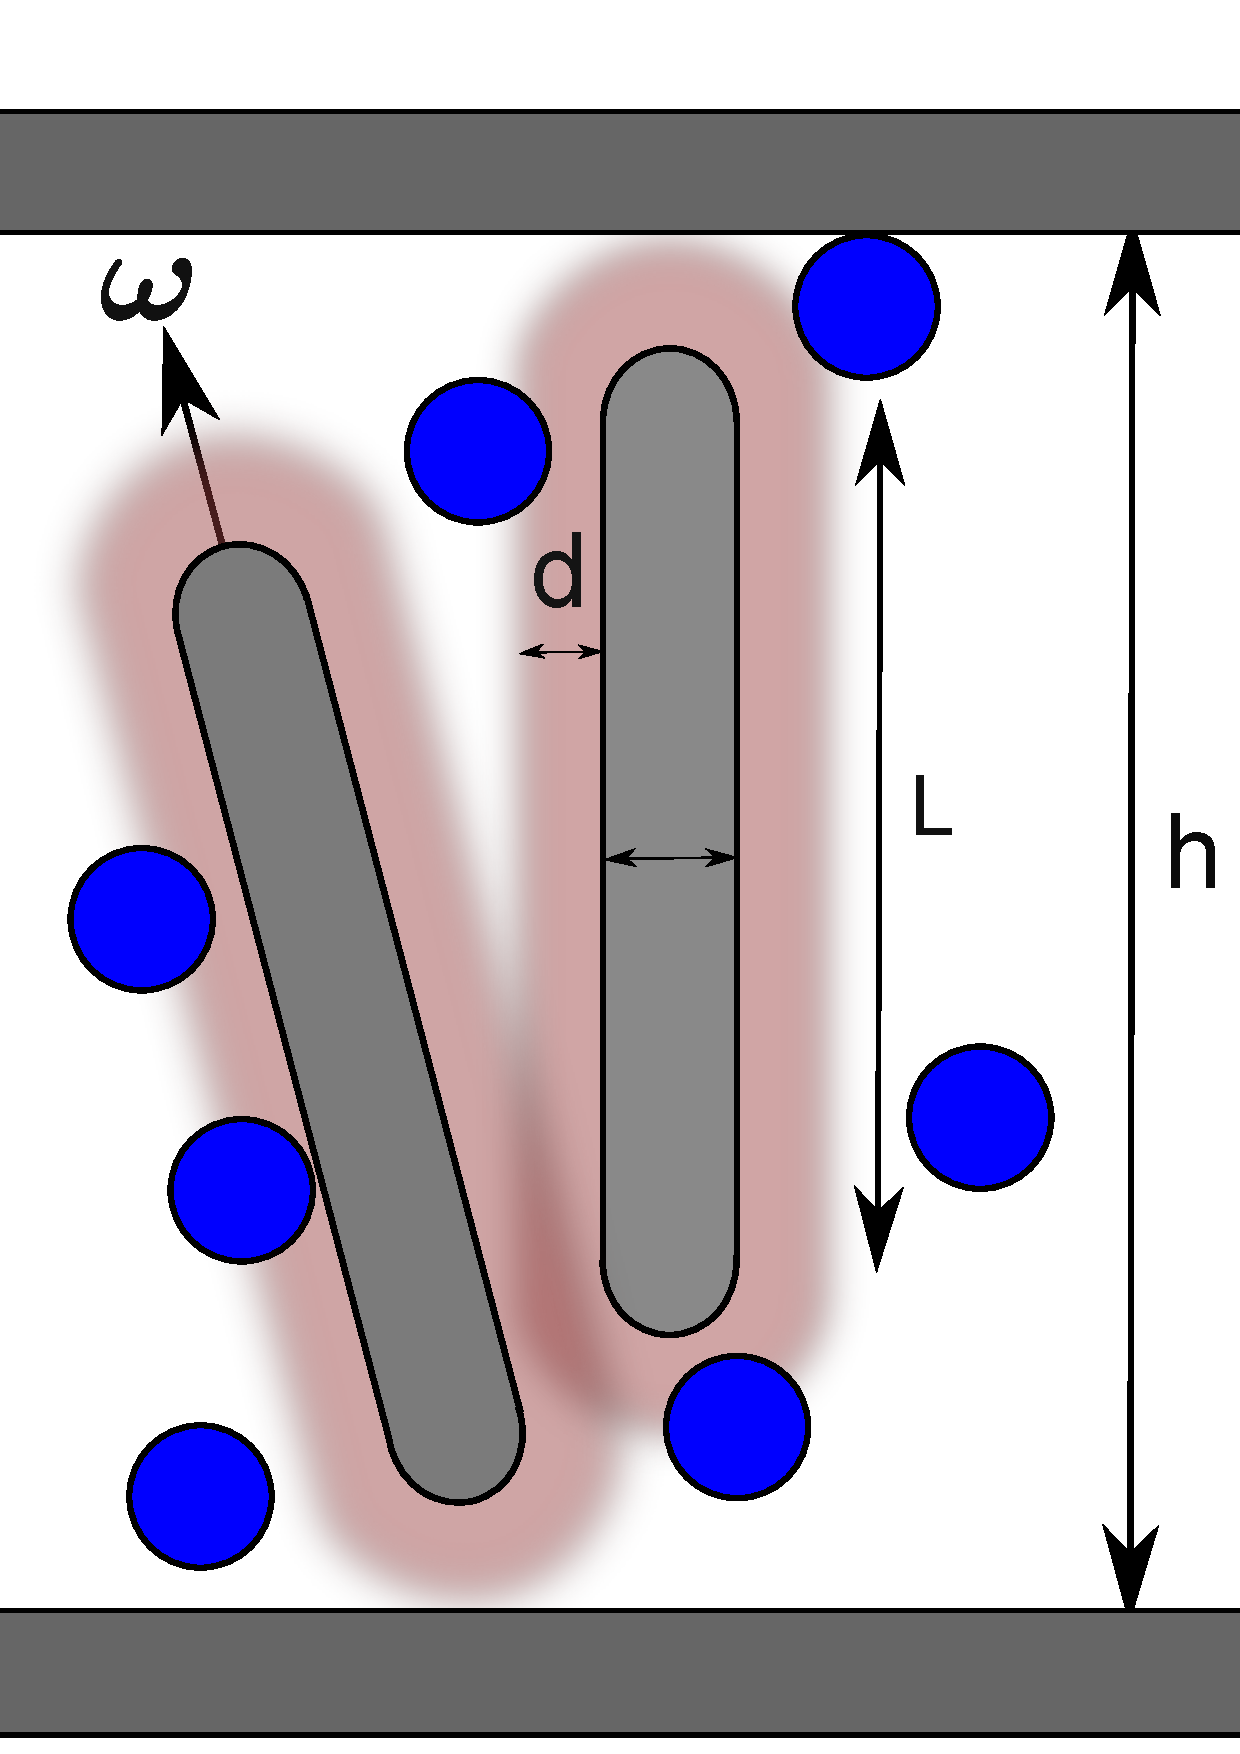
\includegraphics[width = \columnwidth]{figures/chapter-6/spheromans}
	\caption{ Sketch of the simulation model: hard spherocylinders (grey) mixed non-penetrable polymers (blue) with diameter $\sigma = D$ (as depicted here). Overlap of the cores (grey) gives infinite repulsion while overlapping coronae (blurred zones) favors a twisted pair configuration representing the (chiral) electrostatic forces between {\em fd} rods. Two possible setups are considered: (a) The system is in an unconfined environment under periodic boundary conditions. (b) The system is confined in a slab geometry with wall-to-wall distance $h$. Note that this model is defined in (a) two or (b) three spatial dimensions. }
	\label{sketch}
\end{figure}



The pair interaction $U_{r}$ between two spherocylinders with solid angles $\oma$ and $\omb$ and centre-of-mass distance $\Delta \bfr$ follows from a combination of short-range steric forces (treated as strictly hard) and electrostatic forces at larger distance. The  interaction potential between a pair rods depends on centre-of-mass distance vector $\Delta {\bf r}$ and orientation vector $\oma$ of both rods. In our model, the interactions are encapsulated in the following core-shell potential:
\beq
U_{\rm r} (\Delta {\bf r}, \oma, \omb) =
\begin{cases}
\infty & \textrm{if hard cores overlap}\\
U_{\rm twist} & \textrm{otherwise} \\
\end{cases}
\label{urod}
\eeq
The electrostatic interactions between {\em fd} rods gives rise to so-called electrostatic twist which is intimately linked to the chirality surface architecture of {\em fd} virus rods. The chiral  potential is commonly expressed in terms of a pseudoscalar form initially put forward by Goossens:
\beq
U_{\rm twist} (\Delta {\bf r}, \oma , \omb )=
-\varepsilon_{c} \left ( \frac{D}{\Delta r} \right )^{7}(\oma \cdot \omb)(\oma \times \omb \cdot \Delta \hat{\bf r})
\eeq
where  $\Delta \hat{\bf r} $ denotes a unit vector for the centre-of-mass distance.
 The sign of $\varepsilon_{c}$ defines the microscopic handedness of the rods. Without loss of generality we take $\varepsilon_{c} > 0$ reflecting the right-handedness of {\em fd} rods. The chiral symmetry of the potential is expressed by the pseudoscalar that imparts a sign change upon  inversion $\Delta \hat{\bf r} \rightarrow - \Delta \hat{\bf r}$. In view of its rapid decay with $\Delta r$ the potential is very short-ranged and the rods need to be very close together in order to feel the chiral twist.

 %For simplicity, we assume that the twisting forces are sufficiently short-ranged (which should be the case at sufficient ionic strength) and do not  continuously vary with the centre-of-mass distance between the spherocylinders, but are only operative if the coronae between the rods overlap (see \fig{sketch}).


 The typical attraction energy between two rods due to polymer depletion can be estimated from free-volume theory \cite{lekkerkerker2011depletion} and reads:
 \beq
 U_{\rm r,dep} \sim -\Pi_{P} V_{\rm r, ov}
 \eeq
with $ \Pi_{P} = k_{B} T N_{P}/V$ the (van 't Hoff) osmotic pressure of the polymer reservoir and $V_{\rm r, ov}$ the overlap volume  of the depletion layers surrounding each rod which depends on the orientation of each rod. In case the rods are perfectly parallel and at hard-core contact we find a simple analytical result. Ignoring  finite rod size effects we have:
\beq
V_{\rm r, ov} = LD^{2} \left [  2 r^{2} \cos^{-1} \left ( \tfrac{1}{2r} \right )  - \tfrac{1}{2} \sqrt{4 r^{2} -1}  \right ]
\eeq
with $r = \tfrac{1}{2}(1 + \tfrac{\sigma}{D})$. Rescaling in terms of the polymer packing fraction in the reservoir we find that the maximum depletion strength per rod pair  reads:
\beq
  U_{\rm r,dep} \sim - k_{B}T \phi_{P}  \frac{L}{D} \left ( \frac{D}{\sigma} \right )^{3} \left [  2 r^{2} \cos^{-1} \left ( \tfrac{1}{2r} \right )  - \tfrac{1}{2} \sqrt{4 r^{2} -1} \right ]
 \eeq
For a typical set-up ($\phi_{P} =3$, $\sigma = 2D$ and $L/D=10$) this gives about 15 $k_{B}T$ \red{Please verify this}. It is important to keep in mind that the typical energy due to chiral twist should be small ($ | \varepsilon_{c} | \ll U_{\rm r,dep} $) in order to ensure that the cohesive forces among the rods residing in a droplet are dominated by polymer depletion, with chiral twist playing only a perturbative role.


The rods and polymers are confined in a thin slab of width $h = L$ (see \fig{sketch}). The wall-spherocylinder interactions  are strictly hard, that is, infinite repulsion when the spherocylinder core overlaps with the wall and zero repulsion otherwise. More specifically:
\beq
U_{\rm w} (\Delta {\bf r}, \oma) =
\begin{cases}
\infty &  | \Delta {\bf r} \cdot {\bf \hat{n}} | < \frac{L}{2}  | \oma \cdot {\bf \hat{n}} | + \tfrac{D}{2} \\
\infty &   h-  | \Delta {\bf r} \cdot {\bf \hat{n}} | < \frac{L}{2}  | \oma \cdot {\bf \hat{n}} | + \tfrac{D}{2} \\
0 & \textrm{otherwise}
\end{cases}
\label{urodwall}
\eeq
with ${\bf \hat{n} }$ denoting the wall normal.
The polymers do not have any interaction with the wall, but their centres-of-mass are constrained  to reside within the slab.

The simulations are carried out in the semi-grand ensemble, with a fixed number of rods but the polymer content in the system fluctuating against a virtual reservoir consisting of an ideal gas of polymer spheres with a prescribed chemical potential  $\mu_{p}$ which is trivially connected to the polymer packing fraction via:
\beq
\phi_{P} = \frac{\pi D^{3}}{ 6 \Lambda_{p}^{3} } e^{\beta \mu_{P}}
\eeq
where $\Lambda_{P}$ denotes the thermal (de Broglie) wavelength.


Each MC cycle consists of $N + N_{P}$ randomly chosen rod translations, rotations, polymer insertions or removals. The step size for the spherocylinder translations and rotations are chosen adaptively such as to maintain an average acceptance ratio of about 30 \%. The MC code is optimized using cell-linked list routines that significantly reduce the number of overlap checks between rod-rod and rod-polymer pairs involved in  each MC step. \red{Here we need to specify Glaser's cluster move optimization algorithm that we used \cite{glaser2015parallel}.}  We keep a rectangular box shape with $L_{x} = L_{y}$ and $L_{z} = L$ and periodic boundary conditions (PBC) in both lateral directions.

Besides the planar confinement $h$, a further key parameter is the relative strength of chiral twist versus depletion attraction. These can be combined into a dimensionless parameter $\chi_{T}$ balancing the energy scales associated with twist and depletion as previously discussed:
\beq
\chi_{T} = \frac{\varepsilon_{c}}{U_{\rm r, dep}} \ll 1
\eeq
so that twist becomes more prevalent for larger $\chi_{T}$.

Depending on the polymer size the system will either evolve into a liquid drop ("tactoid") or  will retain its crystalline inner structure (expected for `sticky' depletion forces induced by small polymers, $\sigma = D$). We monitor the {\em system} polymer concentration and total twist energy $\mathcal{U}  = \sum_{i}\sum_{j<i}U_{\rm twist}$ to gauge whether or not the drop has reached its equilibrium state.

We plan to focus on two different systems:

\begin{itemize}
\item  i) Small polymers with $\sigma = D$ imparting short-ranged attractions. The initial configuration is a square monolayer of perfectly parallel rods ordered into a hexagonal lattice. Without confinement, the cluster will equilibrate into a membrane with  fluid order. In. our simulations we fix the polymer concentrations $\phi_{P}=1$ and $N=2000$. Note that small changes in $\epsilon_{c}$ may have large consequences for the way the droplet expresses chiral twist. At weak twist ($\varepsilon_{c} < ****$), the membrane remains circular in shape with twist showing up at the membrane edges while the membrane center remains largely unperturbed. At strong twist ($\varepsilon > ****$) the membrane may transform into a twisted ribbon. \red{The first indication of such a change of droplet morphology can be observed in \fig{samples} a and c.   Bigger systems ($N=2000$) spontaneously form ribbon-shaped protrusions around a circular central body which resembles the onset of twisted ribbon formation.  }.  Next we introduce confinement and re-assess the droplet shape and internal structure and compare with experimental observations.

\item ii) Large polymers with $\sigma = 2 D$ imparting long-ranged attractions. We start from the same monolayer crystal which will equilibrate into a liquid tactoid in bulk \cite{kuhnhold2022structure}. Gradually increasing the confinement (at $R_{2} > h$ with $R_{2}$ the minor curvature radius of an unconfined tactoid \cite{kuhnhold2022structure})  will lead to squeezed tactoids which  develop a distinct biaxial shape. Introducing twist may lead to further morphological changes. We may correlate droplet size ($N$) with droplet aspect ratio for the strongly confined case compared to the 3D case studied in \cite{kuhnhold2022structure}.

\end{itemize}


\section{Glaser's Algorithm}

\section{Results}

\begin{figure}
	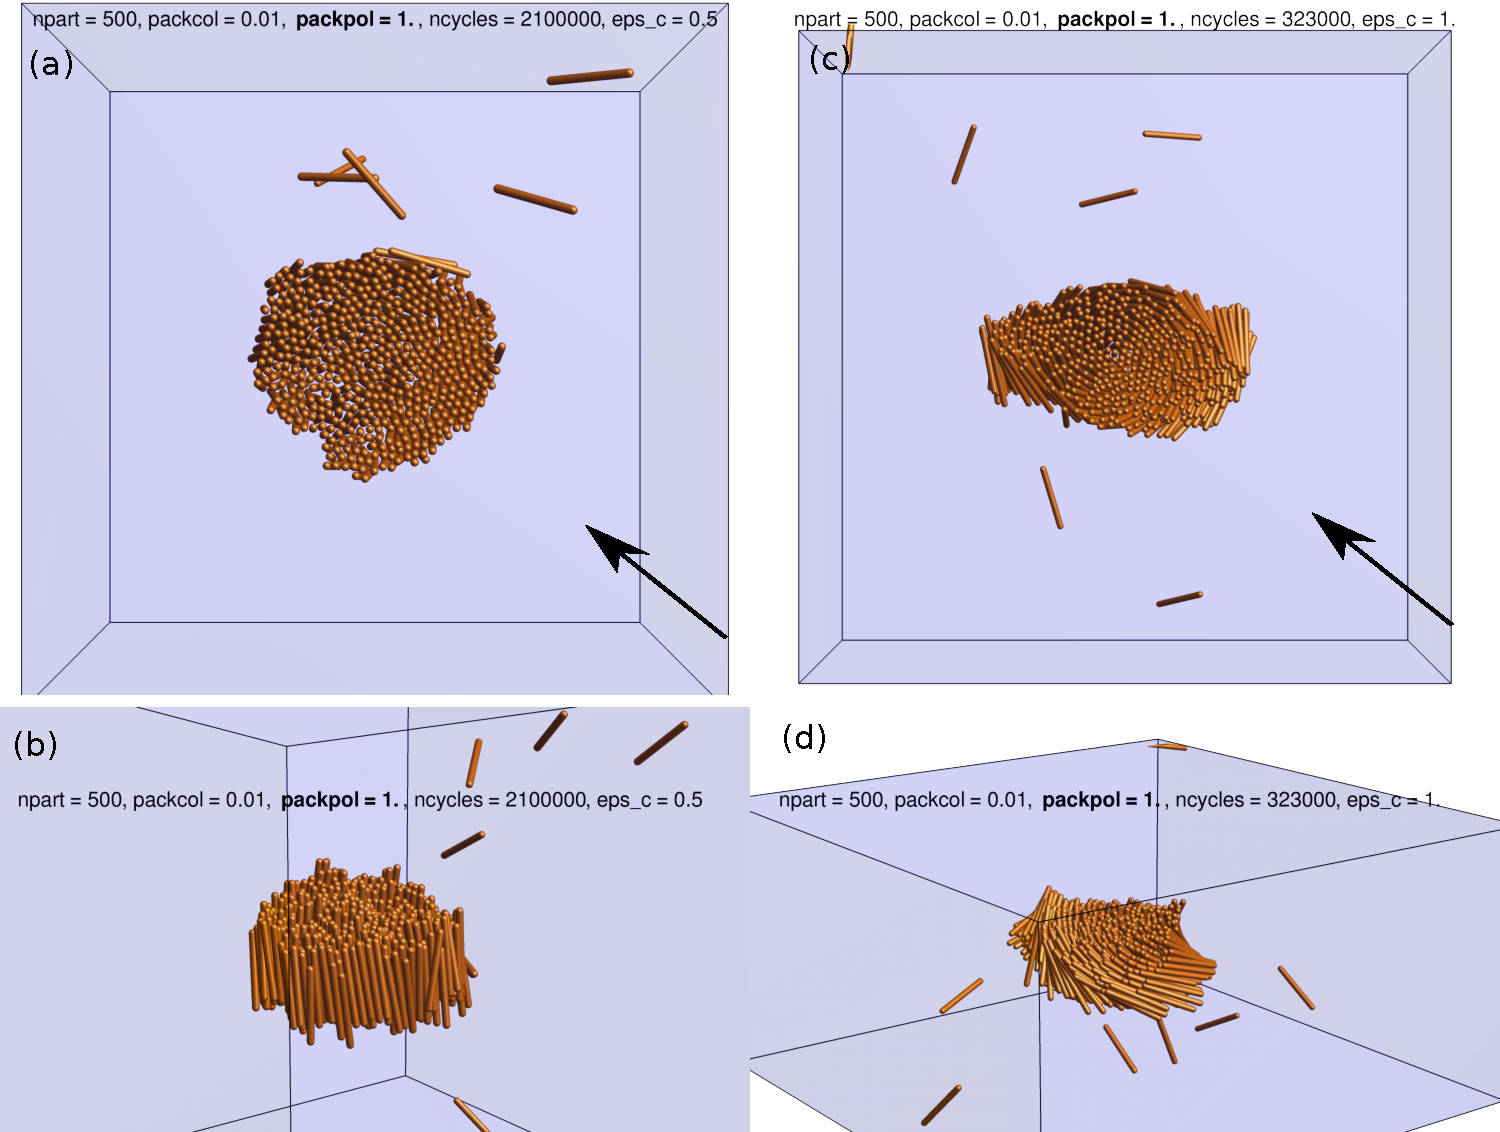
\includegraphics[width = .7\columnwidth]{figures/chapter-6/samples}
	\caption{Membrane-shaped tactoids of chiral rods mixed with non-adsorbing polymer formed in bulk (no confinement). For all runs, $\sigma = D$, chiral radius $d = 0.4D$, $\phi_{P}$ and $N = 500$. (a)-(b) $\varepsilon_{c}=0.5k_BT$, (c)-(d) $\varepsilon_{c}=1k_BT$ Top panels (a),(c) correspond to a top view of the system, bottom panels (b), (d) correspond to a side view with angle indicated by an arrow at the top panels.}
	\label{samples}
\end{figure}

\begin{figure}
	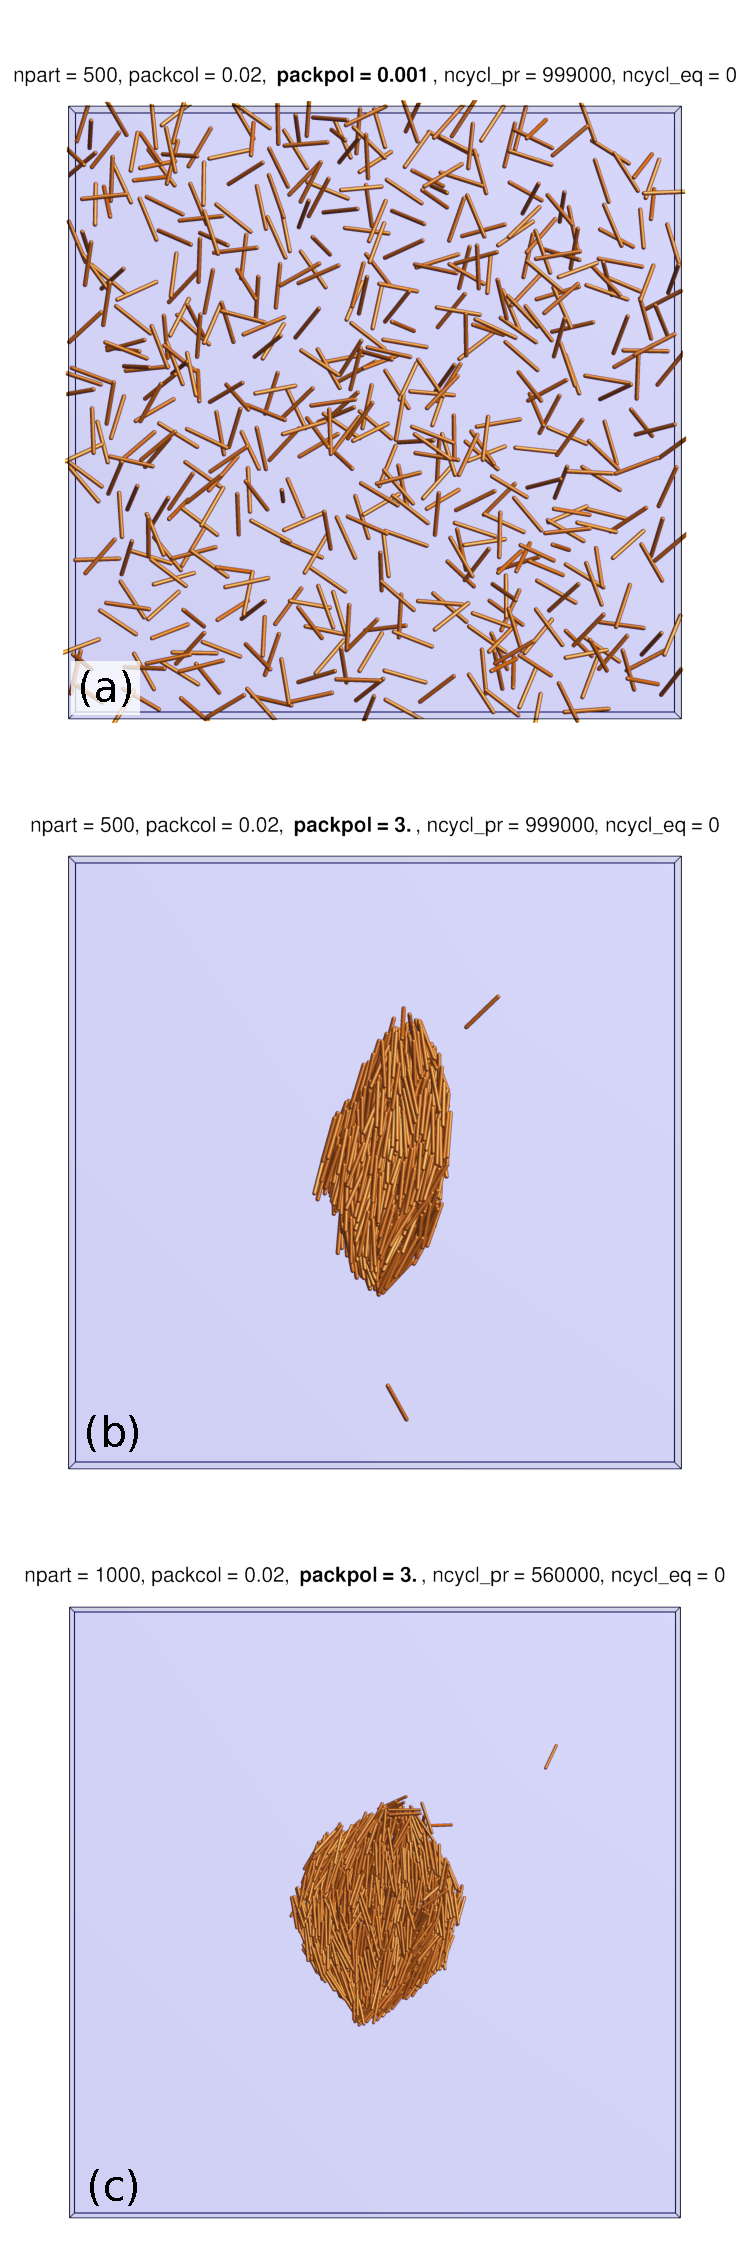
\includegraphics[width = 0.4 \columnwidth]{figures/chapter-6/impl_depletion_effect}
	\caption{ Spindle-shaped tactoids of achiral rods ($\varepsilon_{c}=0$) mixed with non-adsorbing polymer ($\sigma = 2D$) \red{in strong planar confinement ($h = L+D$)}. a) Weak depletion  (very low polymer packing fraction) and $N=500$. b) Strong depletion; $\phi_{P} =3$, $N=500$. c) Strong depletion; $\phi_{P} =3$, $N=1000$. The difference between the shapes between (b) and (c) is explained in \cite{kuhnhold2022structure} for 3-dimensional tactoids: larger nematic droplets tend to be less elongated. The structure in panel (b) is used as an initial configuration in the samples shown in \fig{samples}}
	\label{notwist}
\end{figure}



\clearpage